Nessa tarefa foi simulado a dinâmica de Monte Carlo para sistemas com temperaturas
iniciais relativas à $\beta = 3$ e $\beta = 0.1$. Para temperaturas altas, $\beta$ pequeno, 
é esperado que o sistema não atinja o equílibrio após a dinâmica. O oposto acontece com 
a dinâmica de temperatura baixa, o sistema fica ordenado e a magnetização ficará nula.

As simulação foram feitas para malhas de tamanhos $L = 60$ e $L = 100$. Segue abaixo a estrutura 
a implementação das simulações:

\begin{marginfigure}
    \centering
    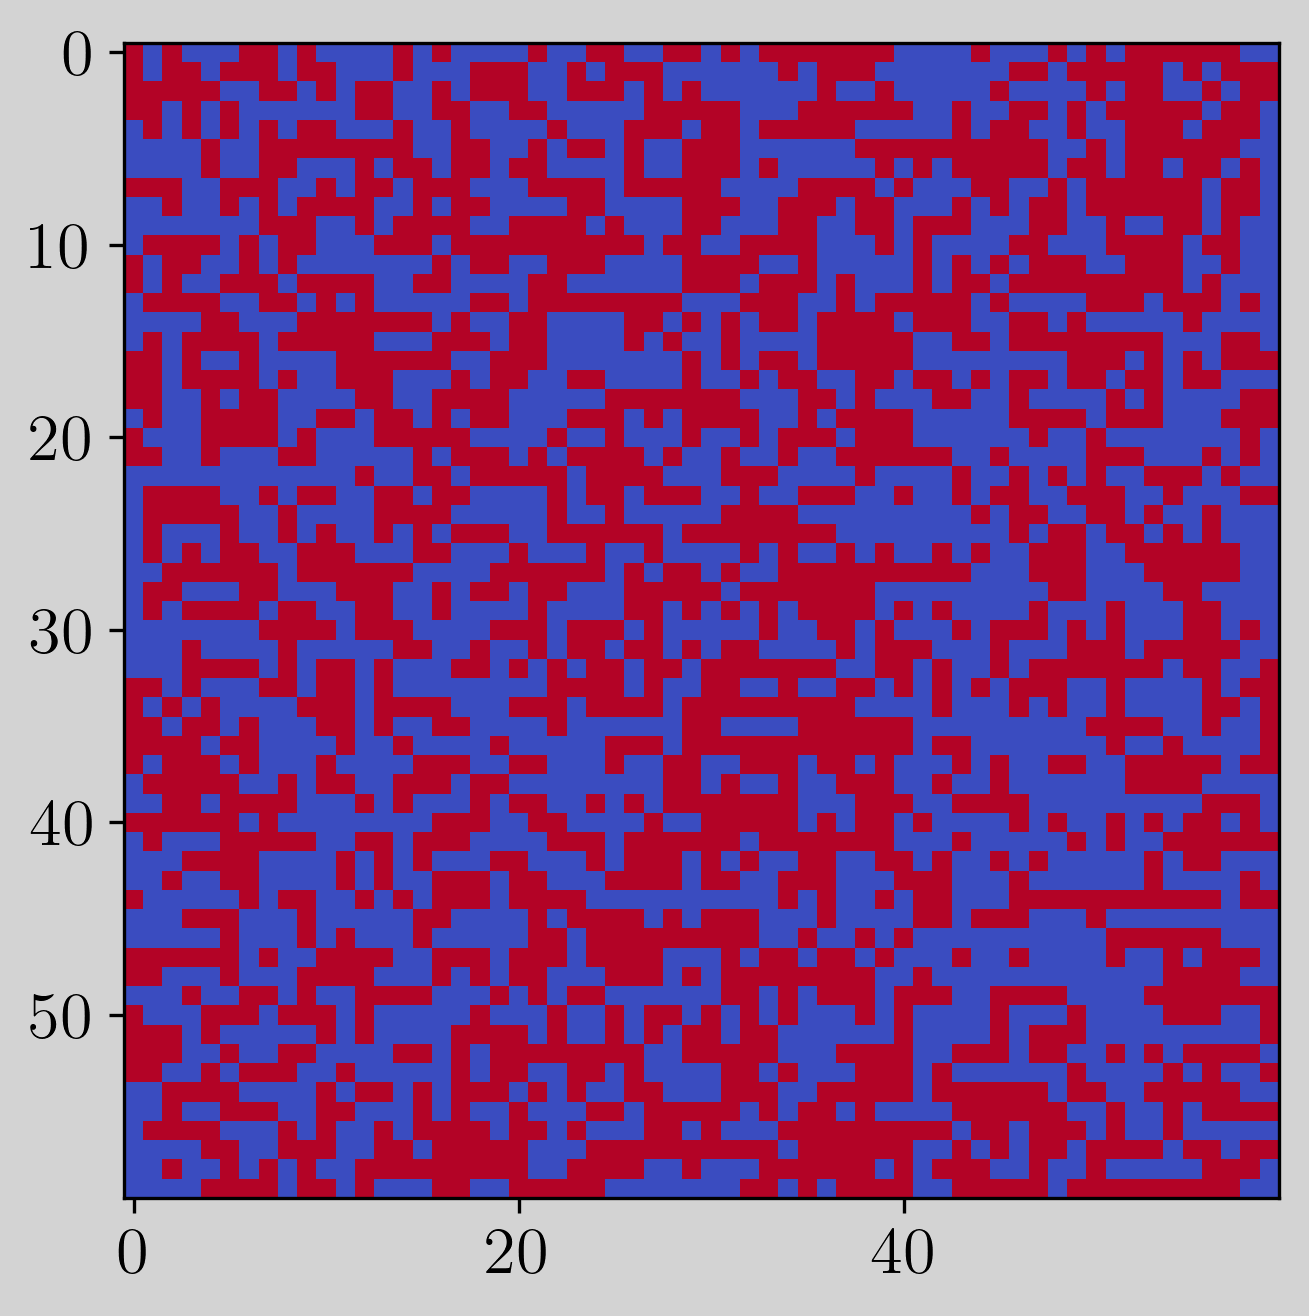
\includegraphics[width=\linewidth]{graficos/tarefa-1/graf-tarefa-A1-conf-L100.png}
    \caption{Configuração final para malha de tamanho $L=100$.}
    \label{fig:a1_l100}
\end{marginfigure}
\begin{minted}{fortran}

    open(1, file="saidas/tarefa-1/saida-tarefa-A1-conf-L60.dat")
    open(3, file="saidas/tarefa-1/saida-tarefa-A1-conf-L100.dat")
    open(5, file="saidas/tarefa-1/saida-tarefa-A2-conf-L60.dat")
    open(7, file="saidas/tarefa-1/saida-tarefa-A2-conf-L100.dat")

    open(2, file="saidas/tarefa-1/saida-tarefa-A1-energia-L60.dat")
    open(4, file="saidas/tarefa-1/saida-tarefa-A1-energia-L100.dat")
    open(6, file="saidas/tarefa-1/saida-tarefa-A2-energia-L60.dat")
    open(8, file="saidas/tarefa-1/saida-tarefa-A2-energia-L100.dat")
    
    call tarefa1(60, 3.0, 1, 2)
    call tarefa1(60, 0.1, 5, 4)

    call tarefa1(100, 3.0, 3, 6)
    call tarefa1(100, 0.1, 7, 8)

    do i = 1, 8
        close(i)    
    end do
    end

    subroutine tarefa1(L_real, beta, fname1, fname2)
        implicit integer(f-f)
        implicit real(m-m)
        parameter(L = 100)

        dimension exps(-4:4)
        byte lattice(1:L, 1:L)
        ! periodic boundary conditions
        dimension ipbc(0:L+1)
        ! this or using mod

        N = L_real * L_real
        ! setting ipbc
        do i = 1, L_real
            ipbc(i) = i
        end do  
        ipbc(0) = L_real
        ipbc(L_real+1) = 1

        m = 0

        call define_exponentials(exps, beta)

        call initialize_lattice(lattice, L_real, L_real)

         ! initial energy
        E = H_0(lattice, ipbc, L_real)

        write(fname2, *) 0, E
        call srand(iseed)
         ! intialize monte carlo dynamics
        do k = 1, 3000
            ! sweeps all configurations
            ! randomly flips spins
            do i = 1 , N
               call flip_spin(lattice,ipbc,exps,E,m,L_real)
            end do  
            write(fname2, *) k, E / N
        end do  
        call write_lattice(lattice, L_real, fname1) 
    end subroutine tarefa1
\end{minted}
\begin{marginfigure}
    \centering
    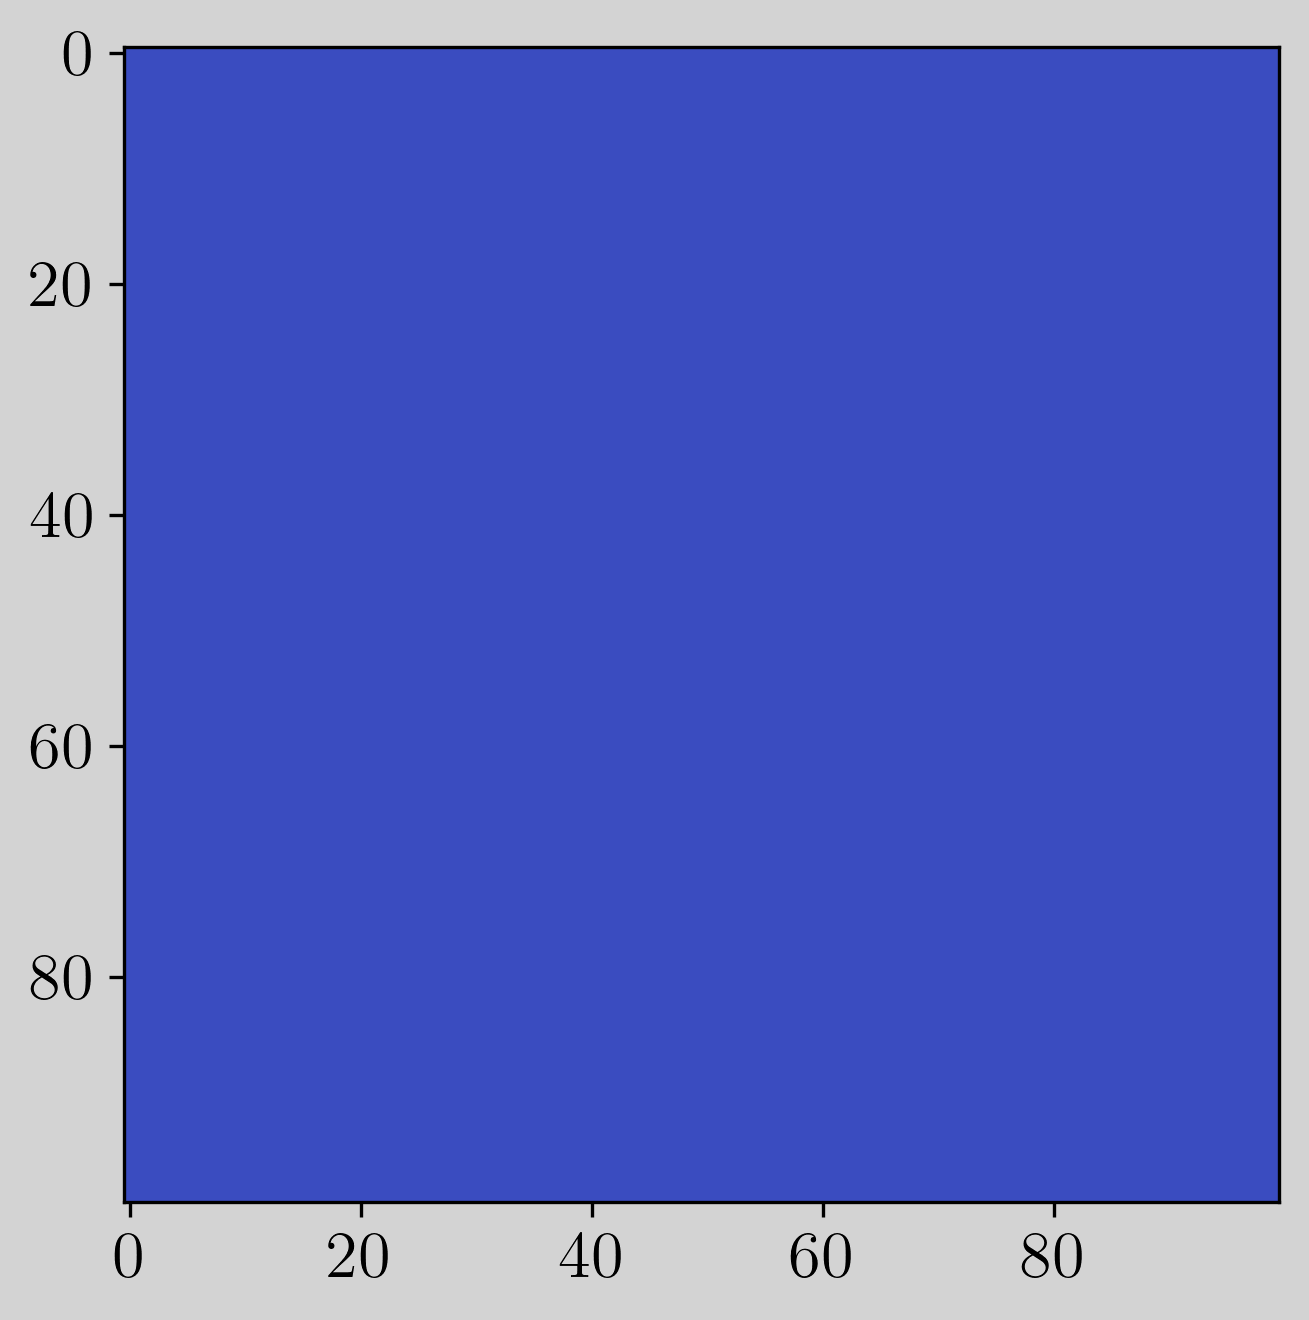
\includegraphics[width=0.6\linewidth]{graficos/tarefa-1/graf-tarefa-A2-conf-L60.png}
    \caption{Configuração final para malha de tamanho L=60.}
\end{marginfigure}

\subsection{A.1 - $\beta = 3$}
Podemos constatar pelas (\ref{fig:a1_l60}) e (\ref{fig:a1_l100}) que o sistema fica totalmente ordenado. 
A magnetização do sistema é $\langle m \rangle = \pm 1$ dependendo da orientação da ordenação. 


% Task 1 Graphs
\begin{marginfigure}
    \centering
    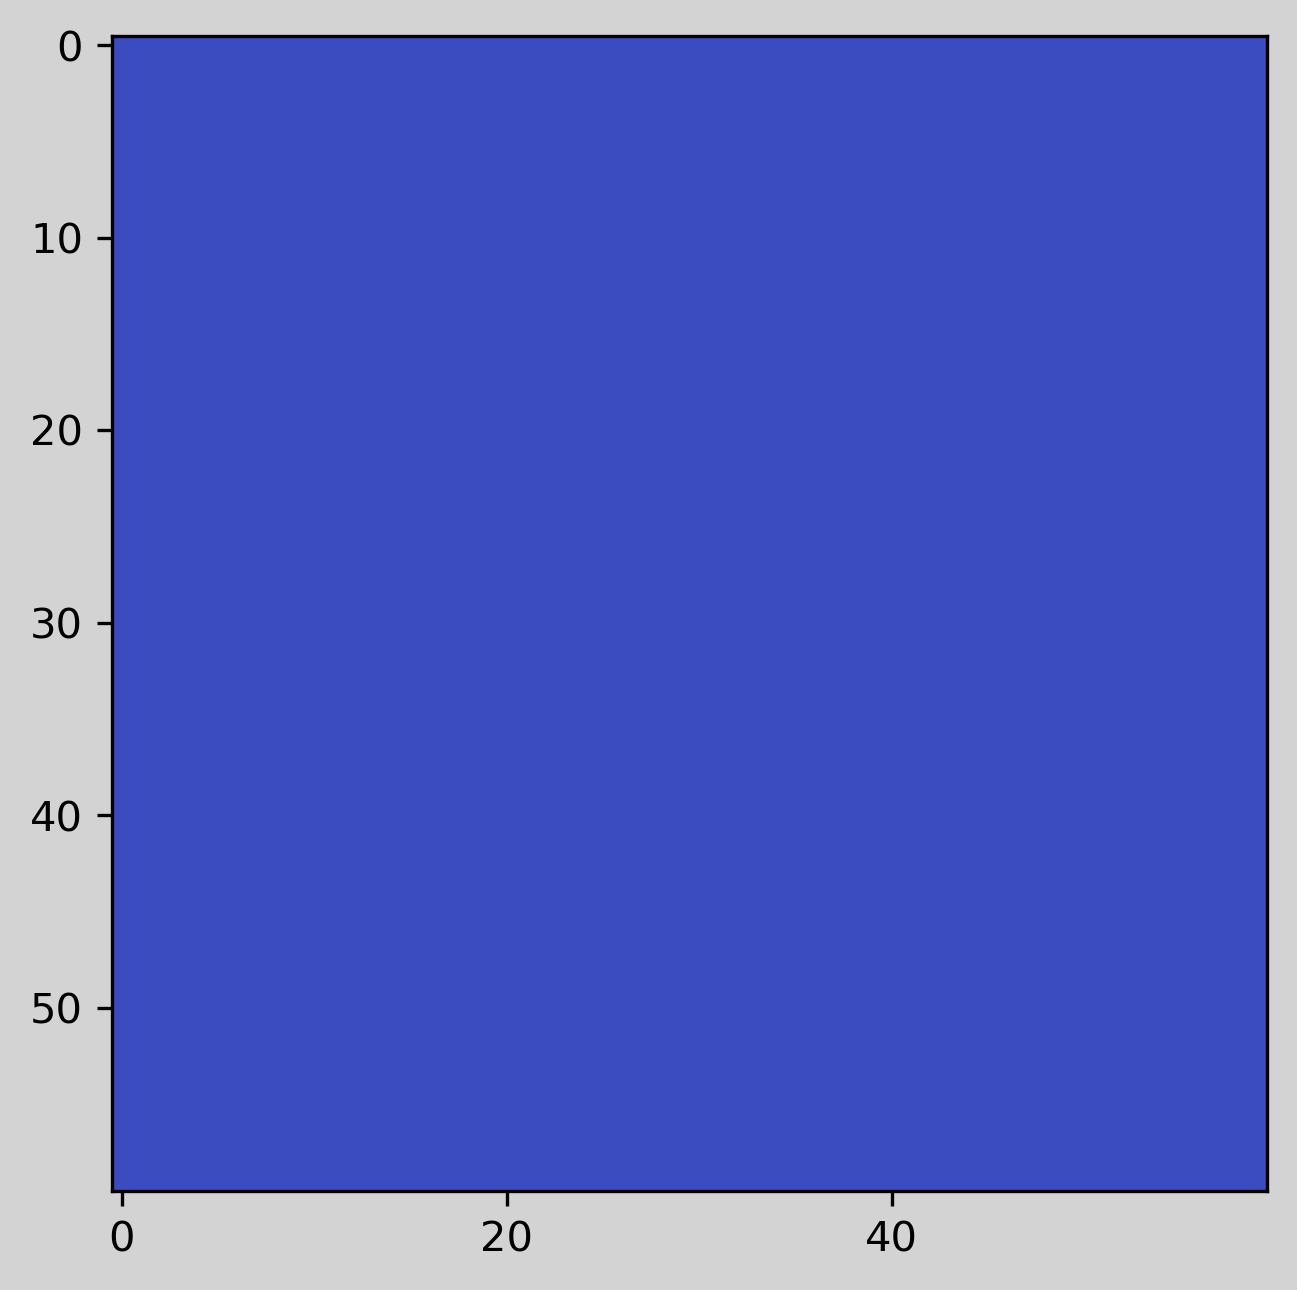
\includegraphics[width=0.6\linewidth]{graficos/tarefa-1/graf-tarefa-A1-conf-L60.png}
    \caption{Configuração final para malha de tamanho $L=60$.}
    \label{fig:a1_l60}
\end{marginfigure}
\subsection{A.2 - $\beta = 0.1$}
Para temperaturas mais altas o sistema fica desordenado, sem uma orientação fixa para
todos spins da malha, nesse caso a simetria vai existir magnetização mas essa é balanceada
pelas orientações contrárias e se cancela. 

Pelas figuras (\ref{fig:a2_l60}) e (\ref{fig:a2_l100}) podemos observar o estado final 
do sistema para diferentes tamanhos de grade.

\begin{marginfigure}[h!]
    \centering
    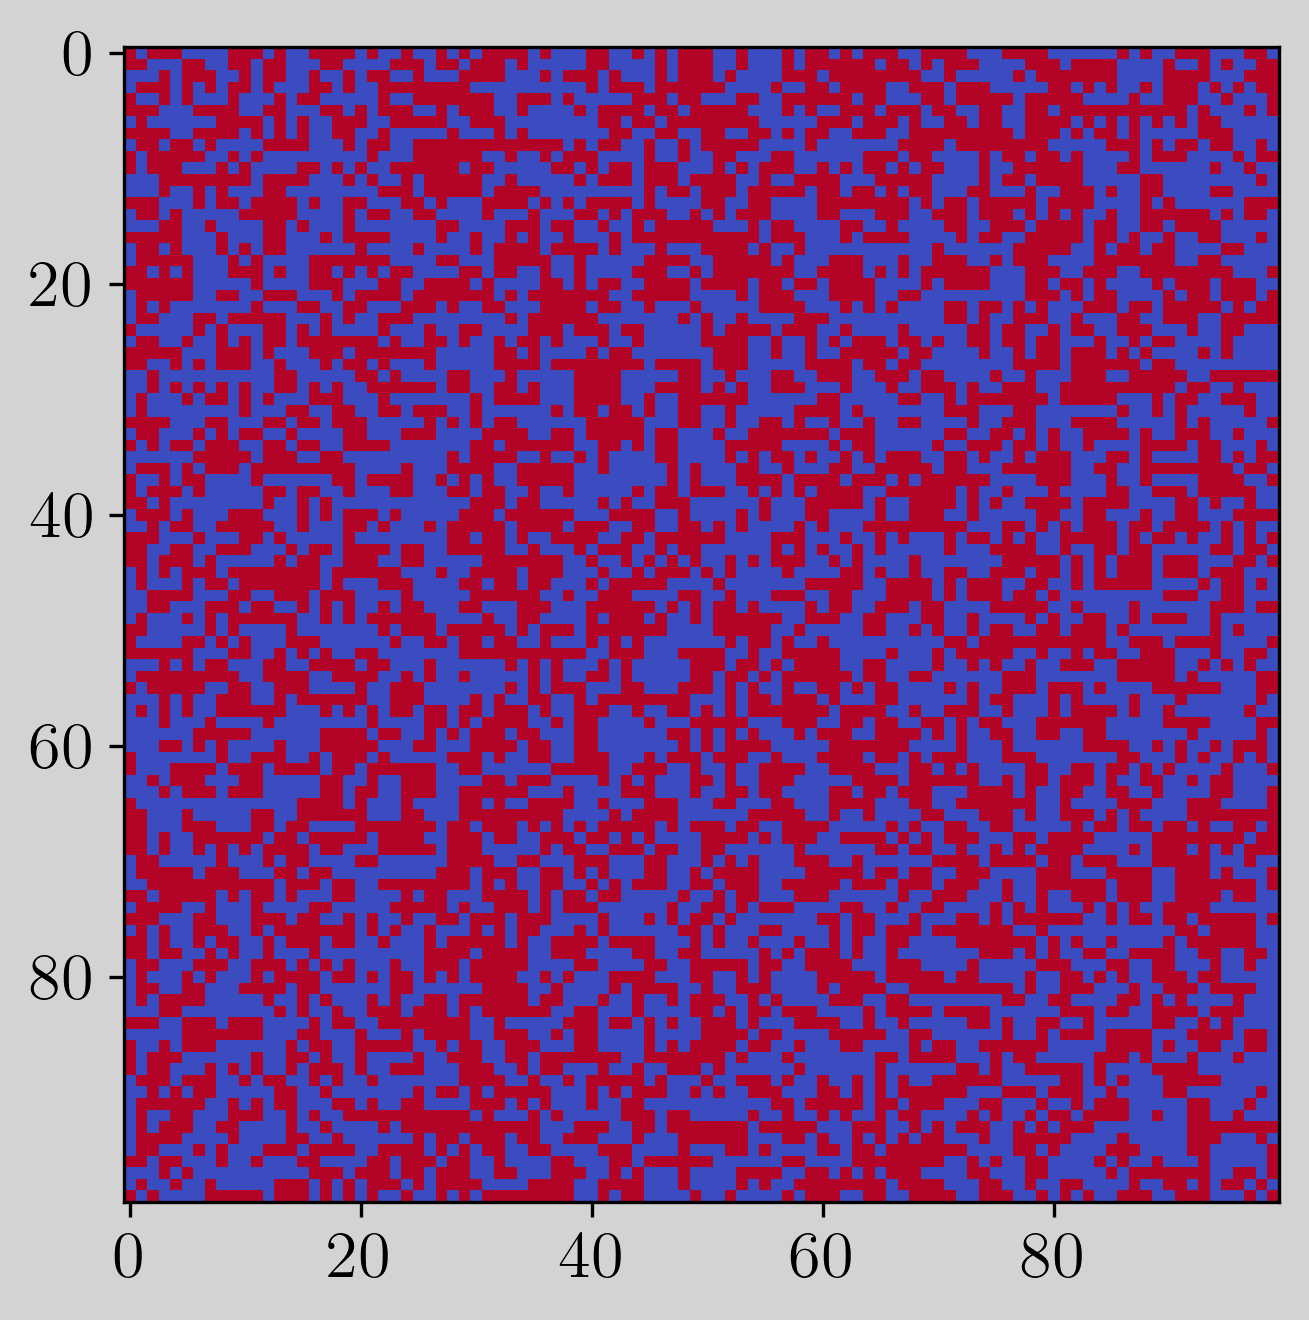
\includegraphics[width=0.7\linewidth]{graficos/tarefa-1/graf-tarefa-A2-conf-L100.png}
    \caption{Configuração inicial para malha de tamanho L=100.}
\end{marginfigure}
